% Author: Rasmus Pank Roulund
\documentclass[tikz]{standalone}

%adapted from http://tex.stackexchange.com/questions/167483/spanning-a-cell-across-several-rows-in-tikz-matrix

\usetikzlibrary{calc,trees,positioning,arrows,chains,shapes.geometric,%
    decorations.pathreplacing,decorations.pathmorphing,shapes,%
    matrix,shapes.symbols,fit}

\pgfdeclarelayer{back}
\pgfsetlayers{back,main}

\tikzstyle{block} = [draw, fill=blue!20, rectangle, 
    minimum height=3em, minimum width=4em]

\tikzstyle{wblock} = [draw, rectangle, 
    minimum height=3em, minimum width=4em]

\makeatletter
\tikzset{
  fitting node/.style={
    inner sep=0pt,
    fill=none,
    draw=none,
    reset transform,
    fit={(\pgf@pathminx,\pgf@pathminy) (\pgf@pathmaxx,\pgf@pathmaxy)}
  },
  reset transform/.code={\pgftransformreset}
}
\makeatother

\begin{document}
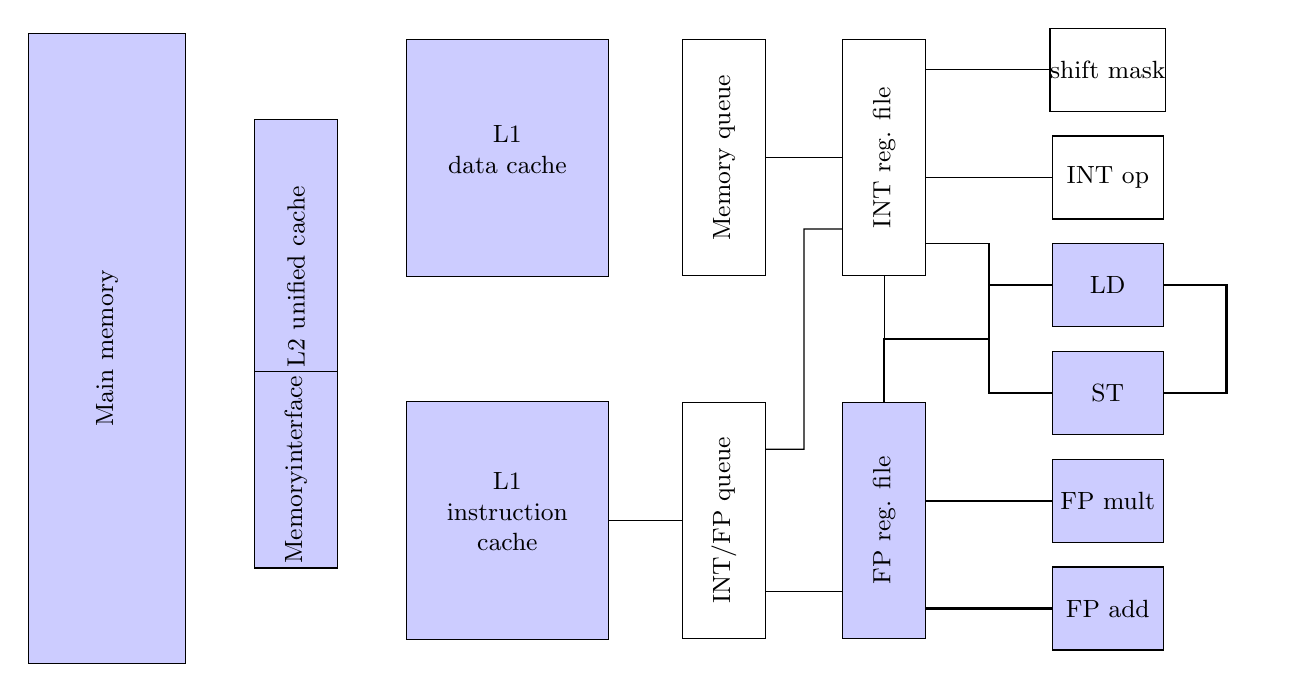
\begin{tikzpicture}[auto, node distance=2.5cm,>=latex',font=\small,
    every node/.style={inner sep=0pt,rectangle, minimum height=2.5em, text centered}]
    \matrix (m) [ampersand replacement=\&,column sep=6mm, row sep=3mm]
    {
      \node (leftof_sm) [coordinate] {}; \& \node (sm) [wblock] {shift\newline{} mask}; \& 
 \\
      \node (leftof_intop) [coordinate] {}; \& \node (intop) [wblock] {INT\newline{} op}; \& 
 \\
      \node (leftof_ld) [coordinate] {}; \& \node (ld) [block] {LD}; \& \node (rightof_ld) [coordinate] {}; \&
 \\
      \node (leftof_st) [coordinate] {}; \& \node (st) [block] {ST}; \& \node (rightof_st) [coordinate] {}; \&
 \\
      \node (leftof_fpmult) [coordinate] {}; \& \node (fpmult) [block] {FP\newline{} mult}; \&
 \\
      \node (leftof_fpadd) [coordinate] {}; \& \node (fpadd) [block] {FP\newline{} add}; \&
 \\
    };

\node (intregfile) [wblock,minimum width=3cm,rotate=90] at($(leftof_intop.west) + (-1.5cm,.25cm)$) {INT reg. file};

\node (fpregfile) [block,rotate=90,minimum width=3cm] at($(leftof_fpmult.west) - (1.5cm,.25cm)$) {FP reg. file};


\path 
let
\p1
 = ($(fpmult.west)$),
\p2
 = ($(fpregfile.south)$),
\p3
 = ($(fpadd.west)$)
in
coordinate
 (fpregfile_hi_right) at (\x2,\y1)
coordinate
 (fpregfile_lo_right) at (\x2,\y3)
;

\draw[thick,-] (fpregfile_hi_right) -- (fpmult.west);
\draw[thick,-] (fpregfile_lo_right) -- (fpadd.west);
\draw[-] (intregfile.west) -- (fpregfile.east);

%\path let \p1 = (A) in node  at (\x1,3) {B};
%\draw (A |- 52,3) node {B};
%\path ($(sm.east)$) edge[-] () ;%

%manual, p.152
\path 
let
\p1
 = ($(sm.west)$),
\p2
 = ($(intregfile.south)$),
\p3
 = ($(intop.west)$),
\p4
 = ($(ld.north)$),
\p5
 = ($(ld.west)$),
\p6
 = ($(st.west)$),
\p7
 = ($(st.east)$),
\n1 = {abs(\x5-\x2)/2},
\n2 = {\x2 + \n1},
\n3 = {\x7 + \n1}
in
coordinate
 (intregfile_hi_right) at (\x2,\y1)
coordinate
 (intregfile_mi_right) at (\x2,\y3)
coordinate
 (intregfile_lo_right) at (\x2,\y4)
coordinate
 (junctn_ld_north) at (\n2,\y4)
coordinate
 (junctn_ld_west) at (\n2,\y5)
coordinate
 (junctn_st_west) at (\n2,\y6)
coordinate
 (junctn_ld_east) at (\n3,\y5)
coordinate
 (junctn_st_east) at (\n3,\y6);

\draw[-] ($(sm.west)$) -- (intregfile_hi_right);
\draw[-] ($(intop.west)$) -- (intregfile_mi_right);
\draw[-] (intregfile_lo_right) -| (junctn_ld_north) -- (junctn_ld_west);
\draw[thick,-] ($(ld.west)$) |- (junctn_ld_west) -- (junctn_st_west) |- ($(st.west)$);

\draw[thick,-] ($(ld.east)$) |- (junctn_ld_east) -- (junctn_st_east) |- ($(st.east)$);
\draw[thick,-] (fpregfile.east) |- ($(fpregfile.east)!.5!(intregfile.west)$) -| ($(junctn_ld_west)!.5!(junctn_st_west)$);


\node (memqueue) [wblock,rotate=90,minimum width=3cm] at($(intregfile.north) - (1.5cm,0cm)$) {Memory queue};
\node (intfpqueue) [wblock,rotate=90,minimum width=3cm] at($(fpregfile.north) - (1.5cm,0cm)$) {INT/FP queue};

\node (ghost1) [coordinate] at($(intregfile.north east)!.8!(intregfile.north west)$) {}; 
\node (leftof_ghost1) [coordinate] at($(memqueue.south east)!.8!(memqueue.south west)$) {}; 
\node (ghost2) [coordinate] at($(fpregfile.north east)!.2!(fpregfile.north west)$) {}; 
\node (leftof_ghost2) [coordinate] at($(intfpqueue.south east)!.2!(intfpqueue.south west)$) {}; 

\path ($(intregfile.north east)!.5!(intregfile.north west)$) edge[-] ($(memqueue.south east)!.5!(memqueue.south west)$) %
($(fpregfile.north east)!.8!(fpregfile.north west)$) edge[-] ($(intfpqueue.south east)!.8!(intfpqueue.south west)$);
\draw[-] ($(intregfile.north east)!.8!(intregfile.north west)$) |- ($(ghost1)!.5!(leftof_ghost1)$) -| ($(ghost2)!.5!(leftof_ghost2)$) -- (leftof_ghost2); %

\draw ([xshift=-3.5cm]memqueue.north east) rectangle ([xshift=-2cm]memqueue.south west) node[fitting node,block] (l1d) {L1\\data cache};

\draw ([xshift=-3.5cm]intfpqueue.north east) rectangle ([xshift=-2cm]intfpqueue.south west) node[fitting node,block] (l1i) {L1\\instruction\\cache};

\path (intfpqueue.north) edge[-] (l1i.east) ;

%\node (l1d) [block,minimum width=3cm] at($(memqueue.north) + (-2.5cm,0.75cm)$) {L1 data cache};
%\node (l1i) [wblock,minimum width=3cm] at($(intfpqueue.north) + (-2.5cm,-0.75cm)$) {L1 instr. cache};


\node (ram) [block,rotate=90,minimum width=8cm, minimum height=2cm] at($(fpadd.west) + (-12.cm,3.3cm)$) {Main memory};

\node (vRAM1) [coordinate] at($(ram.south east)!.4!(ram.south)$) {};
\node (vRAM2) [coordinate] at($(ram.south west)!.4!(ram.south)$) {};

\node (l2cache) [block,rotate=90,minimum width=4cm] at($(l1d.west)!.5!(vRAM1) + (0,-1.5cm)$) {L2 unified cache};
\node (memif) [block,rotate=90,minimum width=2.5cm] at($(l1i.north west)!.5!(vRAM2)$) {Memory\newline{}interface};

% \coordinate (aux1) at (D.west |- A.north);
% \coordinate (aux2) at ($(C.south west) - (3mm,0mm)$);
% \node[block, fit=(aux1)(aux2), inner sep=-.6pt] (X) {}; 
% \node[text width=3cm, text centered, anchor=center, rotate=90] at (X.center) {Main memory};


  \end{tikzpicture}
\end{document}
%%% Local Variables: 
%%% mode: latex
%%% TeX-master: t
%%% End: 
